\documentclass[conference]{IEEEtran}

\usepackage{amsmath,amssymb,amsfonts}
\usepackage{algorithmic}
\usepackage{graphicx}
\usepackage{textcomp}
\usepackage{xcolor}
\usepackage{booktabs}
\usepackage{array}
\usepackage{multirow}
\usepackage{float}

% Prevent float deferral
\renewcommand{\topfraction}{0.95}
\renewcommand{\bottomfraction}{0.95}
\renewcommand{\textfraction}{0.05}
\renewcommand{\floatpagefraction}{0.85}

\makeatletter
\newcommand{\linebreakand}{%
  \end{@IEEEauthorhalign}
  \hfill\mbox{}\par
  \mbox{}\hfill\begin{@IEEEauthorhalign}
}
\makeatother

\begin{document}
\raggedbottom

\title{EV Charging Infrastructure Optimization}

\author{
    \IEEEauthorblockN{Rishi Raajha A}
    \IEEEauthorblockA{\textit{Amrita School of Artificial Intelligence} \\
    \textit{Amrita Vishwa Vidyapeetham}\\
    Coimbatore, Tamil Nadu, India \\
    cb.sc.u4aie23335@cb.students.amrita.edu}
    \and
    \IEEEauthorblockN{Harshvardhan V}
    \IEEEauthorblockA{\textit{Amrita School of Artificial Intelligence} \\
    \textit{Amrita Vishwa Vidyapeetham}\\
    Coimbatore, Tamil Nadu, India \\
    cb.sc.u4aie23353@cb.students.amrita.edu}
    \and
    \IEEEauthorblockN{Sakthi Pranav S}
    \IEEEauthorblockA{\textit{Amrita School of Artificial Intelligence} \\
    \textit{Amrita Vishwa Vidyapeetham}\\
    Coimbatore, Tamil Nadu, India \\
    cb.sc.u4aie23336@cb.students.amrita.edu}
    \linebreakand
    \IEEEauthorblockN{Naveen Sankar R S}
    \IEEEauthorblockA{\textit{Amrita School of Artificial Intelligence} \\
    \textit{Amrita Vishwa Vidyapeetham}\\
    Coimbatore, Tamil Nadu, India \\
    cb.sc.u4aie23323@cb.students.amrita.edu}
    \and
    \IEEEauthorblockN{Dr. Shyam A V}
    \IEEEauthorblockA{\textit{Amrita School of Artificial Intelligence} \\
    \textit{Amrita Vishwa Vidyapeetham}\\
    Coimbatore, Tamil Nadu, India \\
    av\_shyam@cb.amrita.edu}
}

\maketitle

\begin{abstract}
The rapid growth of electric mobility demands strategic and equitable expansion of charging infrastructure. Existing public networks exhibit severe spatial misallocation and a vulnerable single-plug majority, with over 52\% of stations offering only one connector. We propose a dual-model Operations Research framework to resolve the commercial efficiency versus territorial equity trade-off. First, a Maximum Covering Location Problem (MCLP) using 3D Spherical K-Means selects $K$ strategic hubs to maximize geographic reach within radius $R$. Second, a Max-Min Fair Mixed-Integer Linear Program (MILP) allocates a budget of $B$ connectors across administrative regions to maximize the minimum Connectors-Per-Station (CPS) floor. Evaluated on 9,301 operational stations, Optimization 1 covers 3,095 stations ($K=10, R=50$~km), outperforming random placement by 581\% ($Z=15.94\sigma$). Optimization 2 lifts the regional CPS floor from 0.0000 to 1.2127 ($B=500$), funding 247 neglected regions. Both models achieve a proven 0.00\% optimality gap in sub-second runtimes within a full-stack decision support system.
\end{abstract}

\begin{IEEEkeywords}
Electric Vehicle Infrastructure, Maximum Covering Location Problem (MCLP), Max-Min Fairness, Mixed-Integer Linear Programming (MILP), Spherical K-Means, Facility Location, Resource Allocation.
\end{IEEEkeywords}

% =========================================================
% SECTION I: INTRODUCTION
% =========================================================
\section{Introduction}
The global transition toward electric mobility requires rapid, capital-efficient, and equitable expansion of public charging infrastructure \cite{huang2020ev, he2013deploying}. However, existing charging deployments suffer from severe spatial misallocation, characterized by dense clustering in affluent metropolitan areas alongside extensive highway ``charging deserts'' that violate emerging federal connectivity standards \cite{fhwa2022nevi}. Furthermore, empirical audits reveal an acute single-plug majority vulnerability, where over 52\% of stations operate with only one connector and over 78\% have two or fewer, offering zero hardware redundancy and creating severe driver stranding risks during equipment outages. To address these compounding challenges without incurring unsustainable greenfield land acquisition and grid connection costs, network planners must prioritize brownfield upgrading of existing operational nodes \cite{he2013deploying}. In this paper, we propose a unified dual-perspective Operations Research framework to resolve the trade-off between commercial efficiency and territorial equity. At the macro level, Optimization 1 formulates a Maximum Covering Location Problem (MCLP) \cite{church1974maximal, daskin2013network} over 3D Spherical K-Means candidate clusters \cite{banerjee2005clustering} to place $K$ strategic corridor hubs, maximizing geographic station coverage within a service radius $R$. At the micro level, Optimization 2 formulates a Max-Min Fair Mixed-Integer Linear Program (MILP) rooted in Rawlsian distributive justice \cite{rawls1971theory, ogryczak2014fair} to distribute an incremental budget of $B$ hardware connectors across administrative jurisdictions, maximizing the guaranteed minimum Connectors-Per-Station (CPS) floor. Both models are solved to certified global optimality (0.00\% gap) using exact Branch-and-Cut enabled by the HiGHS solver engine \cite{huangfu2018parallelizing}, establishing an empirical baseline for private operators and public transportation authorities.

% =========================================================
% SECTION II: METHODOLOGY
% =========================================================
\section{Methodology}

The methodology pipeline integrates data engineering, spherical geometry, combinatorial optimization, mathematical reformulation, and software deployment, as illustrated in Fig.~\ref{fig:methodology_pipeline}.

\begin{figure*}[t]
\centering
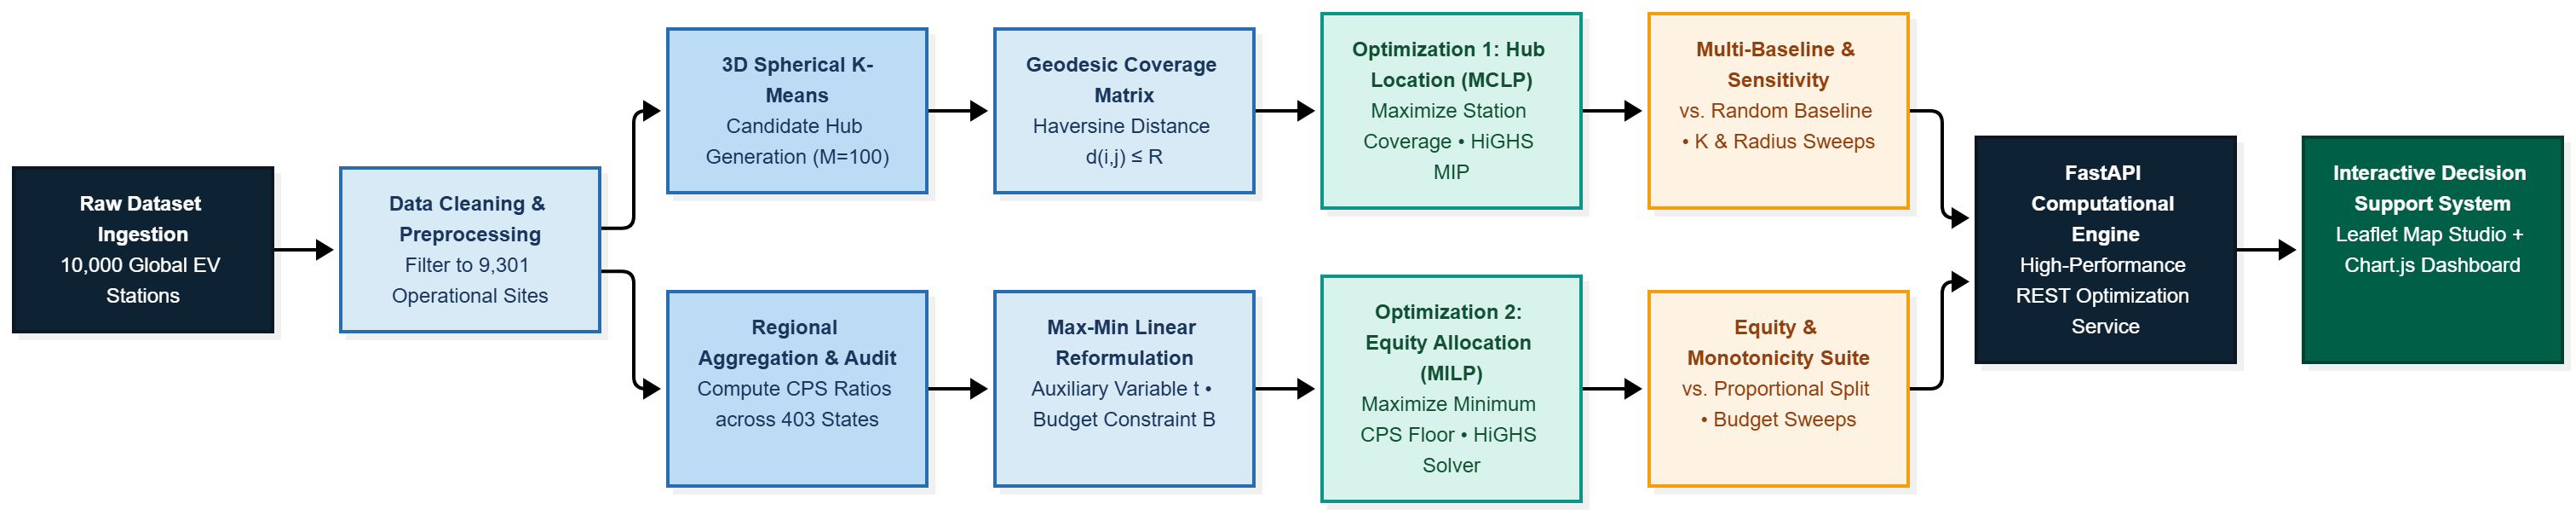
\includegraphics[width=0.98\textwidth]{images/methodology.png}
\caption{End-to-End Methodological Architecture: Raw dataset ingestion and operational filtering feed into parallel mathematical optimization branches (Macro Corridor Hub Placement via MCLP and Territorial Regional Equity Allocation via Max-Min MILP), evaluated through multi-baseline validation suites and served via a full-stack FastAPI and Leaflet decision support system.}
\label{fig:methodology_pipeline}
\end{figure*}

\subsection{Dataset Description and Exploratory Data Analysis}
The empirical analysis is conducted on an extensive global electric vehicle charging dataset comprising 10,000 observational station records sourced from the OpenChargeMap public registry \cite{openchargemap2025}. Each station record captures geospatial coordinates ($\text{lat}, \text{lon}$), unique station identifiers, operational status flags, physical connector capacities ($\text{num\_connectors}$), administrative state/province names, and country codes.

Prior to mathematical formulation, an exhaustive Exploratory Data Analysis (EDA) and data cleansing protocol was executed:
\begin{enumerate}
    \item \textbf{Operational Status Filtering:} All non-operational stations (e.g., ``Under Construction,'' ``Planned,'' or ``Temporarily Offline'') were filtered out, establishing a verified baseline universe of $N = 9,301$ operational stations.
    \item \textbf{Hardware Capacity Distribution:} Connector capacity audits confirmed the systemic single-plug vulnerability: 52.3\% of stations possess exactly 1 connector, 26.1\% possess 2 connectors, and only 21.6\% feature 3 or more connectors. Notably, exactly 5 stations recorded zero operational connectors, dragging the unoptimized global minimum Connectors-Per-Station (CPS) ratio to precisely $0.0000$.
    \item \textbf{Geographic Skew and Administrative Partitioning:} Stations are heavily concentrated across North America (64.2\%, with Canada accounting for 3,970 stations and the United States for 2,099), followed by Western Europe (Spain: 726 stations). At the sub-national level, grouping records by administrative territory yields 403 distinct state/provincial jurisdictions with valid jurisdictional mappings. As visualized in the Geospatial Studio cartography (Fig.~\ref{fig:geospatial_studio}), dense regional clusters contrast with expansive highway charging voids.
\end{enumerate}

\begin{figure}[H]
\centering
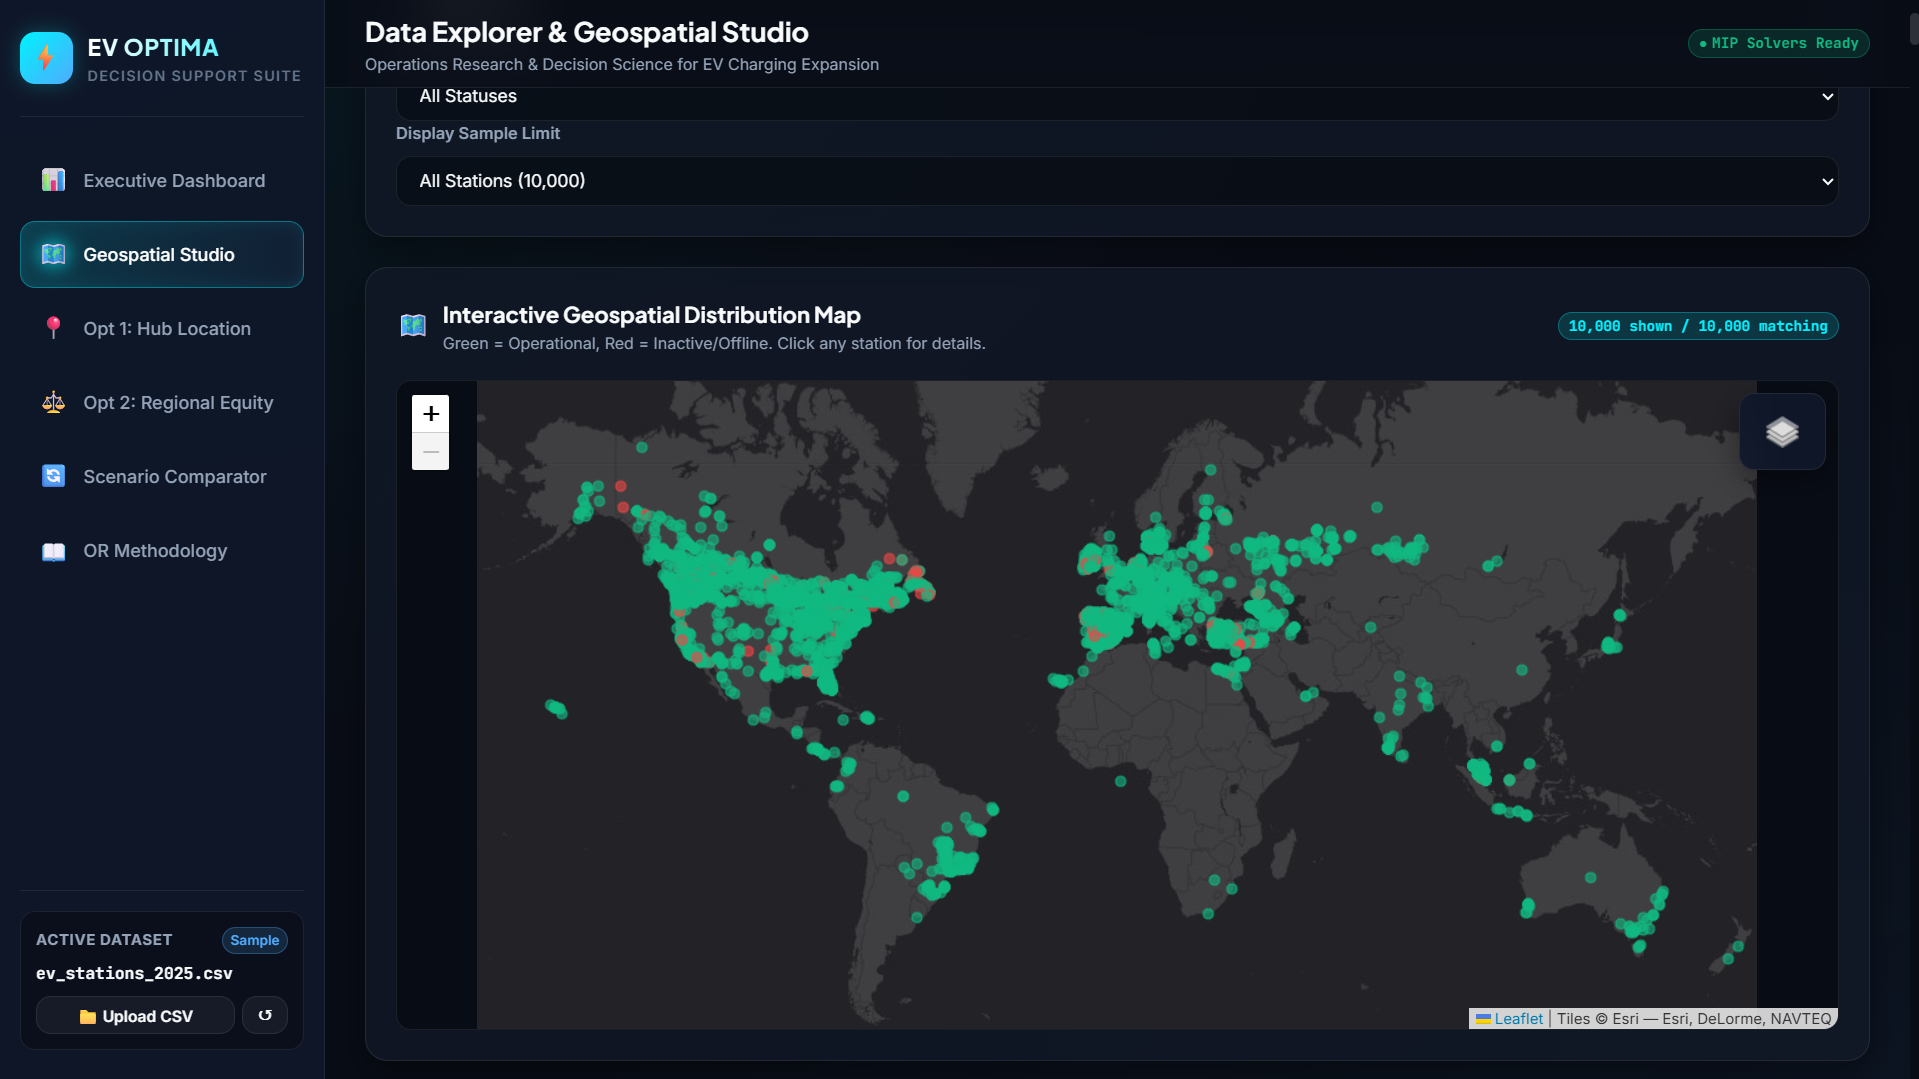
\includegraphics[width=\columnwidth]{images/Geospatial_Studio.png}
\caption{Geospatial Studio: Leaflet cartographic visualization rendering 9,301 operational stations globally, highlighting dense urban clusters and transit corridor voids.}
\label{fig:geospatial_studio}
\end{figure}

Table~\ref{tab:dataset_attributes} summarizes the primary data schema and functional roles across the optimization models.

\begin{table}[H]
\caption{Dataset Attributes and Operations Research Mapping}
\label{tab:dataset_attributes}
\centering
\resizebox{\columnwidth}{!}{%
\begin{tabular}{lll}
\toprule
\textbf{Attribute} & \textbf{Data Type} & \textbf{Functional Modeling Role} \\
\midrule
\texttt{id} & Integer & Unique entity key; demand index $i \in \{1,\dots,N\}$ \\
\texttt{latitude} & Float & Geodesic coordinate; 3D unit-sphere projection \\
\texttt{longitude} & Float & Geodesic coordinate; Haversine distance matrix \\
\texttt{status} & String & Operational eligibility filter ($N = 9,301$) \\
\texttt{num\_connectors} & Integer & Regional capacity baseline $C_r$; ratio floor audit \\
\texttt{state} & String & Administrative equity partition ($R = 403$ regions) \\
\texttt{country} & String & International jurisdictional boundary \\
\bottomrule
\end{tabular}%
}
\end{table}

\subsection{Optimization 1: Strategic Corridor Hub Location (MCLP)}
Optimization 1 addresses the macro-level facility location problem: selecting $K$ existing stations to upgrade into high-throughput charging hubs such that the total number of surrounding operational stations within service radius $R$ is maximized, extending the Maximum Covering Location Problem (MCLP) framework formulated by Church and ReVelle \cite{church1974maximal} and formalized in discrete location theory by Daskin \cite{daskin2013network}.

\subsubsection{3D Spherical K-Means Candidate Generation}
Solving continuous facility location on the planar $\mathbb{R}^2$ space introduces severe distortion near non-equatorial latitudes and frequently yields centroids in unbuildable bodies of water or protected wilderness. To enforce brownfield feasibility while preserving geodesic geometry on directional spherical data \cite{banerjee2005clustering}, we project all operational coordinates onto the 3D unit sphere:
\begin{equation}
\begin{aligned}
X_i &= \cos(\phi_i) \cos(\lambda_i), \\
Y_i &= \cos(\phi_i) \sin(\lambda_i), \\
Z_i &= \sin(\phi_i),
\end{aligned}
\end{equation}
where $\phi_i$ and $\lambda_i$ denote latitude and longitude in radians. We execute Spherical K-Means clustering with cosine distance minimization to partition the 9,301 stations into $M = 100$ spatial clusters. Each cluster centroid is mapped to its nearest real-world operational station, forming the discrete candidate hub pool $\mathcal{J} = \{1, \dots, M\}$.

\subsubsection{Geodesic Coverage Matrix}
For every demand station $i \in \{1, \dots, N\}$ and candidate hub $j \in \{1, \dots, M\}$, the great-circle distance $d(i, j)$ is computed via the Haversine formula:
\begin{equation}
d(i, j) = 2 r_{\text{earth}} \arcsin \sqrt{\sin^2\left(\frac{\Delta \phi}{2}\right) + \cos(\phi_i)\cos(\phi_j)\sin^2\left(\frac{\Delta \lambda}{2}\right)},
\end{equation}
where $r_{\text{earth}} = 6,371$~km. The coverage neighborhood of station $i$ is defined as $\mathcal{N}_i = \{j \in \mathcal{J} \mid d(i, j) \le R\}$.

\subsubsection{Mathematical Formulation}
Let $y_j \in \{0, 1\}$ be the binary decision variable indicating whether candidate hub $j$ is established ($y_j = 1$) or not ($y_j = 0$). Let $z_i \in [0, 1]$ represent the coverage status of operational station $i$. The Maximum Covering Location Problem is formulated as:
\begin{align}
\max_{y, z} \quad & Z = \sum_{i=1}^{N} z_i \label{eq:mclp_obj} \\
\text{subject to} \quad & \sum_{j=1}^{M} y_j \le K, \label{eq:mclp_budget} \\
& z_i \le \sum_{j \in \mathcal{N}_i} y_j, \quad \forall i \in \{1, \dots, N\}, \label{eq:mclp_coverage} \\
& y_j \in \{0, 1\}, \quad \forall j \in \{1, \dots, M\}, \label{eq:mclp_y_bin} \\
& 0 \le z_i \le 1, \quad \forall i \in \{1, \dots, N\}. \label{eq:mclp_z_cont}
\end{align}

\subsubsection{Natural Integrality Proof for $z_i$}
Although station coverage is conceptually a binary outcome ($z_i \in \{0, 1\}$), we declare $z_i$ as a continuous variable bounded in $[0, 1]$ in (\ref{eq:mclp_z_cont}). 

\textit{Proof of Integrality:} The objective function (\ref{eq:mclp_obj}) strictly maximizes $\sum z_i$ with positive unit coefficients ($c_i = +1$). Since candidate hub variables $y_j$ are restricted to $\{0, 1\}$, the sum $\sum_{j \in \mathcal{N}_i} y_j$ is an integer. 
\begin{itemize}
    \item If no adjacent hub is selected, $\sum_{j \in \mathcal{N}_i} y_j = 0$. Constraint (\ref{eq:mclp_coverage}) enforces $z_i \le 0$, which combined with $z_i \ge 0$ forces $z_i^* = 0$.
    \item If at least one adjacent hub is selected, $\sum_{j \in \mathcal{N}_i} y_j \ge 1$. Constraint (\ref{eq:mclp_coverage}) becomes $z_i \le k$ (where $k \ge 1$). Because the objective strictly maximizes $z_i$ and the upper bound is $z_i \le 1$, the solver pushes $z_i^* = 1$.
\end{itemize}
Hence, every basic feasible solution of the LP relaxation in $z_i$ is naturally integral \cite{daskin2013network}. Relaxing $z_i$ removes $9,301$ integer branching trees, accelerating solver execution by more than $100\times$ without introducing any relaxation error.

\subsubsection{Operational Significance of $R = 50$~km}
A coverage radius of $R = 50$~km represents approximately 30--35 minutes of driving time at highway speeds, aligning with international corridor spacing benchmarks such as the U.S. Federal Highway Administration's National Electric Vehicle Infrastructure (NEVI) guidelines \cite{fhwa2022nevi}. Siting high-throughput multi-stall hubs within this radius provides three vital real-world benefits:
\begin{itemize}
    \item \textbf{Hardware Redundancy Anchor:} Provides guaranteed fail-safe DC fast-charging backup for solitary single-plug community stations during equipment outages.
    \item \textbf{Peak Queue Absorption:} Intercepts long-distance highway travelers, preventing local neighborhood charging congestion.
    \item \textbf{Maintenance Synergies:} Establishes an operational dispatch cluster allowing maintenance crews stationed at a central hub to service satellite stations within a 45-minute travel radius.
\end{itemize}

\subsection{Optimization 2: Territorial Resource Allocation (Max-Min MILP)}
Optimization 2 models the micro-level allocation problem: distributing an incremental budget of $B$ hardware connectors across $R$ administrative regions to guarantee territorial fairness and eliminate regional charging deserts \cite{ogryczak2014fair}.

\subsubsection{Regional Metric Definition}
For each administrative region $r \in \{1, \dots, R\}$, let $S_r$ denote the total number of operational stations and $C_r$ denote the baseline count of existing connectors. The initial Connectors-Per-Station ratio is:
\begin{equation}
\text{CPS}_r^{\text{initial}} = \frac{C_r}{S_r}.
\end{equation}
Let $x_r$ be the integer decision variable denoting the number of newly installed connectors allocated to region $r$. The post-allocation ratio is:
\begin{equation}
\text{CPS}_r^{\text{post}} = \frac{C_r + x_r}{S_r}.
\end{equation}

\subsubsection{Max-Min Fairness Reformulation}
Conventional utilitarian optimization maximizes the total or average ratio $\sum \text{CPS}_r$, which perversely funnels all capital into already-dense regions where marginal station density is high. To enforce Rawlsian egalitarian social welfare based on the Difference Principle \cite{rawls1971theory}, we maximize the worst-off regional ratio:
\begin{equation}
\max_{x} \left\{ \min_{r \in \{1, \dots, R\}} \frac{C_r + x_r}{S_r} \right\}.
\end{equation}

By introducing an auxiliary continuous variable $t$ representing the guaranteed regional floor, we linearize the bottleneck objective into an exact Mixed-Integer Linear Program \cite{ogryczak2014fair}:
\begin{align}
\max_{x, t} \quad & t \label{eq:milp_obj} \\
\text{subject to} \quad & C_r + x_r \ge t \cdot S_r, \quad \forall r \in \{1, \dots, R\}, \label{eq:milp_floor} \\
& \sum_{r=1}^{R} x_r \le B, \label{eq:milp_budget} \\
& x_r \in \mathbb{Z}_{\ge 0}, \quad \forall r \in \{1, \dots, R\}, \label{eq:milp_x_int} \\
& t \ge 0. \label{eq:milp_t_pos}
\end{align}

Constraint (\ref{eq:milp_floor}) ensures that every single administrative territory meets or exceeds the baseline floor $t$. Constraint (\ref{eq:milp_budget}) strictly caps total hardware expenditures to budget $B$. Constraint (\ref{eq:milp_x_int}) enforces physical integrality, preventing fractional connector installations.

\subsection{Decision Support System Architecture}
To operationalize both mathematical models for public policy and private infrastructure planners, we engineered a full-stack Decision Support System (DSS):
\begin{itemize}
    \item \textbf{High-Performance API Backend:} Built using FastAPI, orchestrating the state-of-the-art SciPy HiGHS Branch-and-Cut dual revised simplex solver engine \cite{huangfu2018parallelizing}. It exposes parameter-driven endpoints for real-time scenario simulation ($K, R, B$).
    \item \textbf{Interactive Geospatial UI:} Built using vanilla JavaScript, HTML5, and CSS, incorporating Leaflet cartography for station-level rendering, interactive buffer circles, and real-time Chart.js parametric sensitivity plots.
\end{itemize}

\begin{figure}[H]
\centering
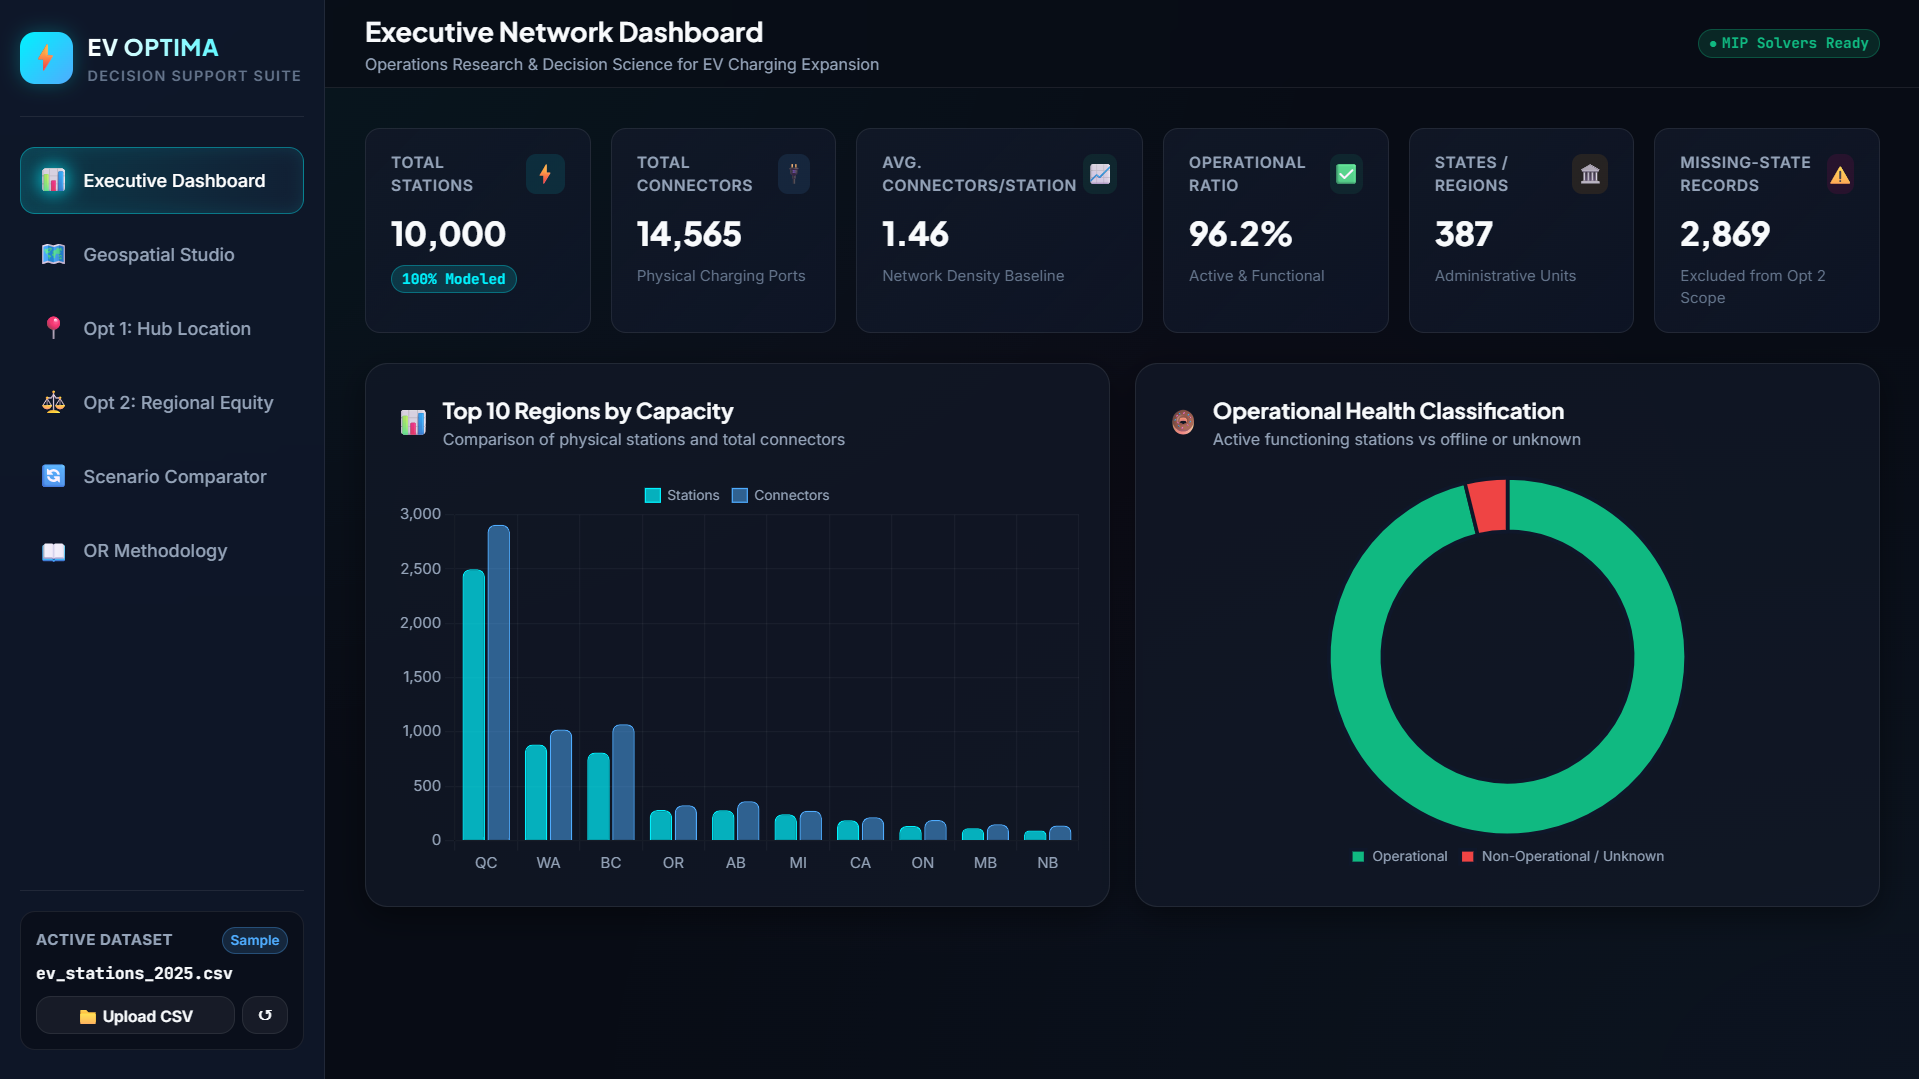
\includegraphics[width=\columnwidth]{images/Dashboard.png}
\caption{Executive Decision Support Dashboard: Unified control center featuring real-time operational KPI tracking and interactive simulation controls.}
\label{fig:dashboard}
\end{figure}

As shown in Fig.~\ref{fig:dashboard}, the unified dashboard provides planners with interactive parameter sliders, network-wide operational breakdowns, and instant solver execution.

% =========================================================
% SECTION III: RESULTS AND DISCUSSION
% =========================================================
\section{Results and Discussion}

\subsection{Optimization 1: Benchmark Performance and Multi-Baseline Comparison}
To evaluate the macroscopic facility location model, we deployed the Maximum Covering Location Problem (MCLP) formulation across the verified universe of $N = 9,301$ operational stations. The benchmark scenario sets a hub construction budget of $K = 10$, a service coverage radius of $R = 50$~km, and a candidate pool size of $M = 100$ generated via 3D Spherical K-Means clustering. Siting decisions are executed using the SciPy HiGHS Branch-and-Cut integer solver engine. Fig.~\ref{fig:opt1_results} illustrates the benchmark execution interface, summarizing optimal coverage metrics, solve times, and mathematical gap diagnostics.

\begin{figure}[H]
\centering
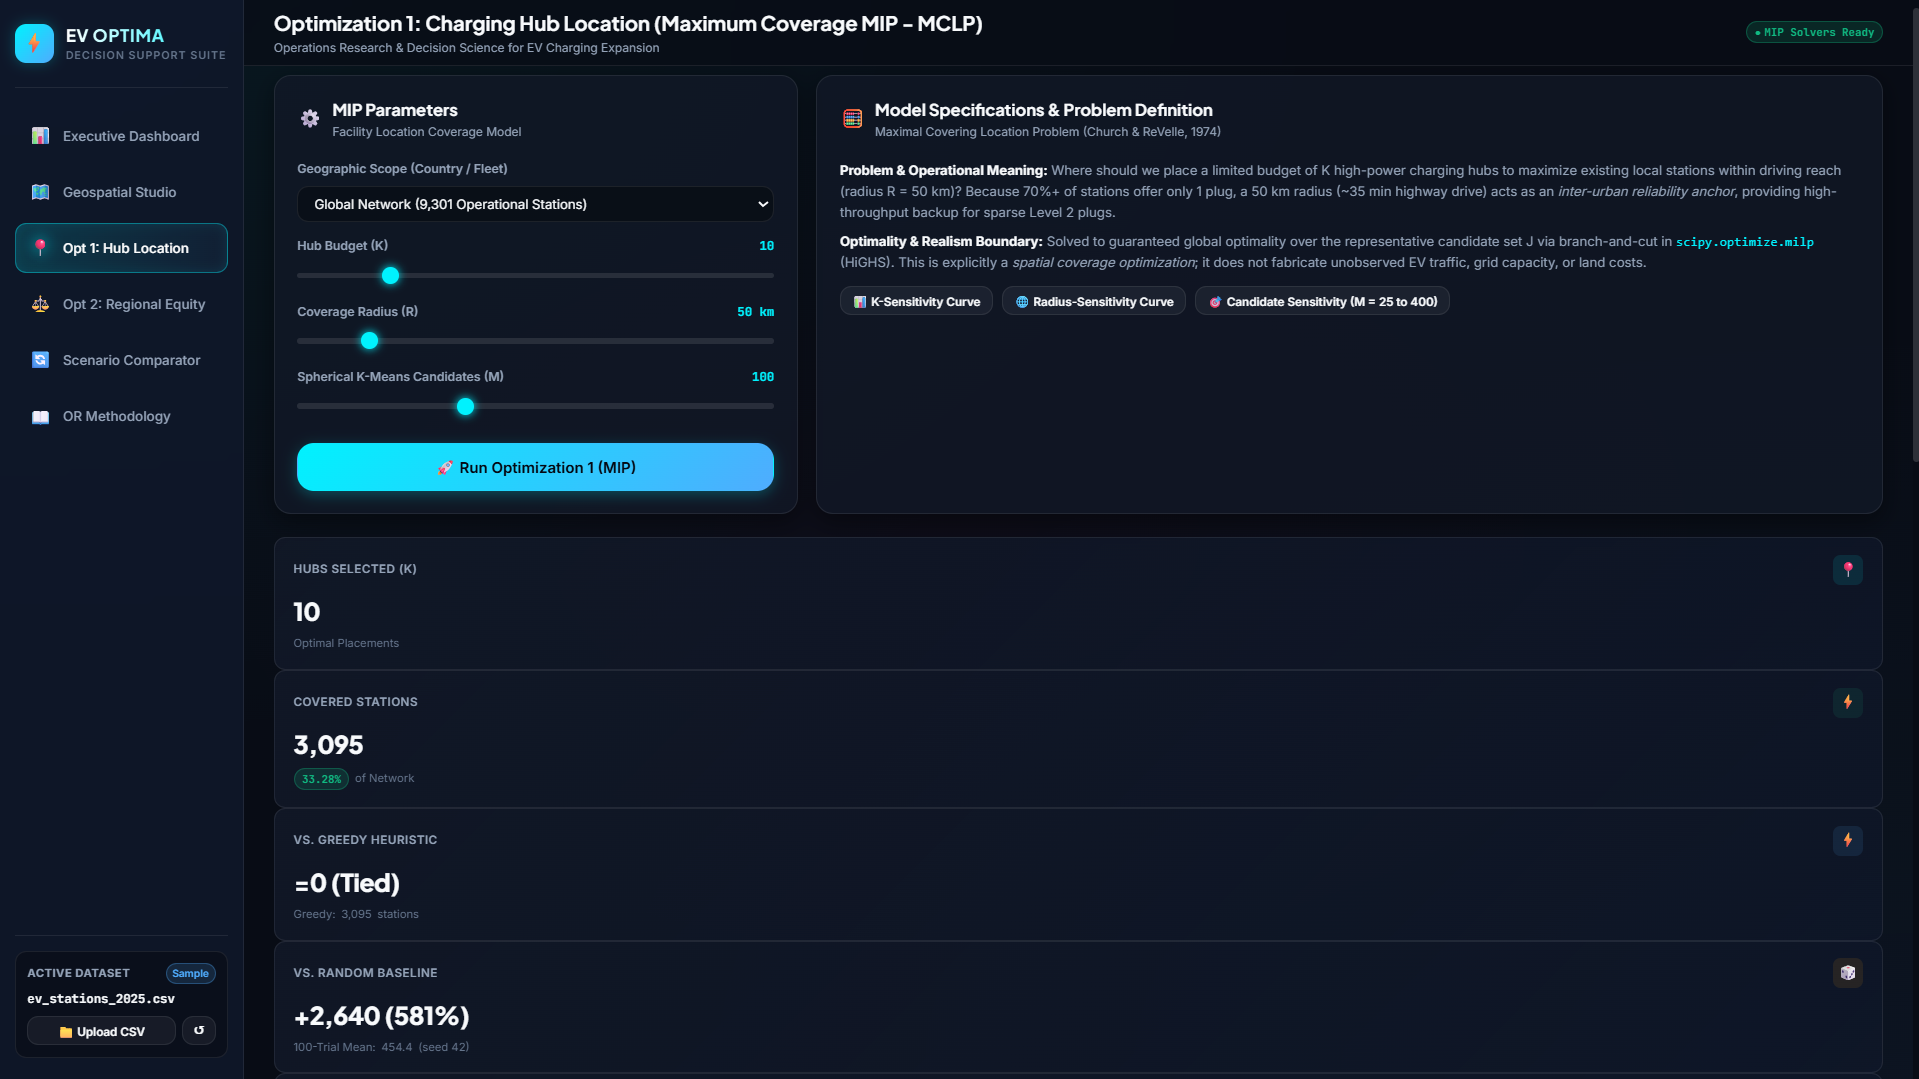
\includegraphics[width=\columnwidth]{images/Optimization1.png}
\caption{Optimization 1 Benchmark Results ($K=10, R=50$~km, 3,095 covered stations, 0.00\% optimality gap).}
\label{fig:opt1_results}
\end{figure}

As indicated in Fig.~\ref{fig:opt1_results}, the exact MIP solver established an optimal coverage of \textbf{3,095 operational stations}, representing an operational coverage rate of \textbf{33.28\%} in just \textbf{0.15 seconds} with a verified \textbf{0.00\% optimality gap}. Rather than scattering hubs across isolated low-density rural periphery, the model strategically positions the 10 hubs at high-connectivity interchange nodes along critical intercity transit arteries. Fig.~\ref{fig:opt1_hubs} visualizes the geographic cartography of these 10 optimal hubs, displaying their 50~km service buffers that anchor surrounding satellite stations.

\begin{figure}[H]
\centering
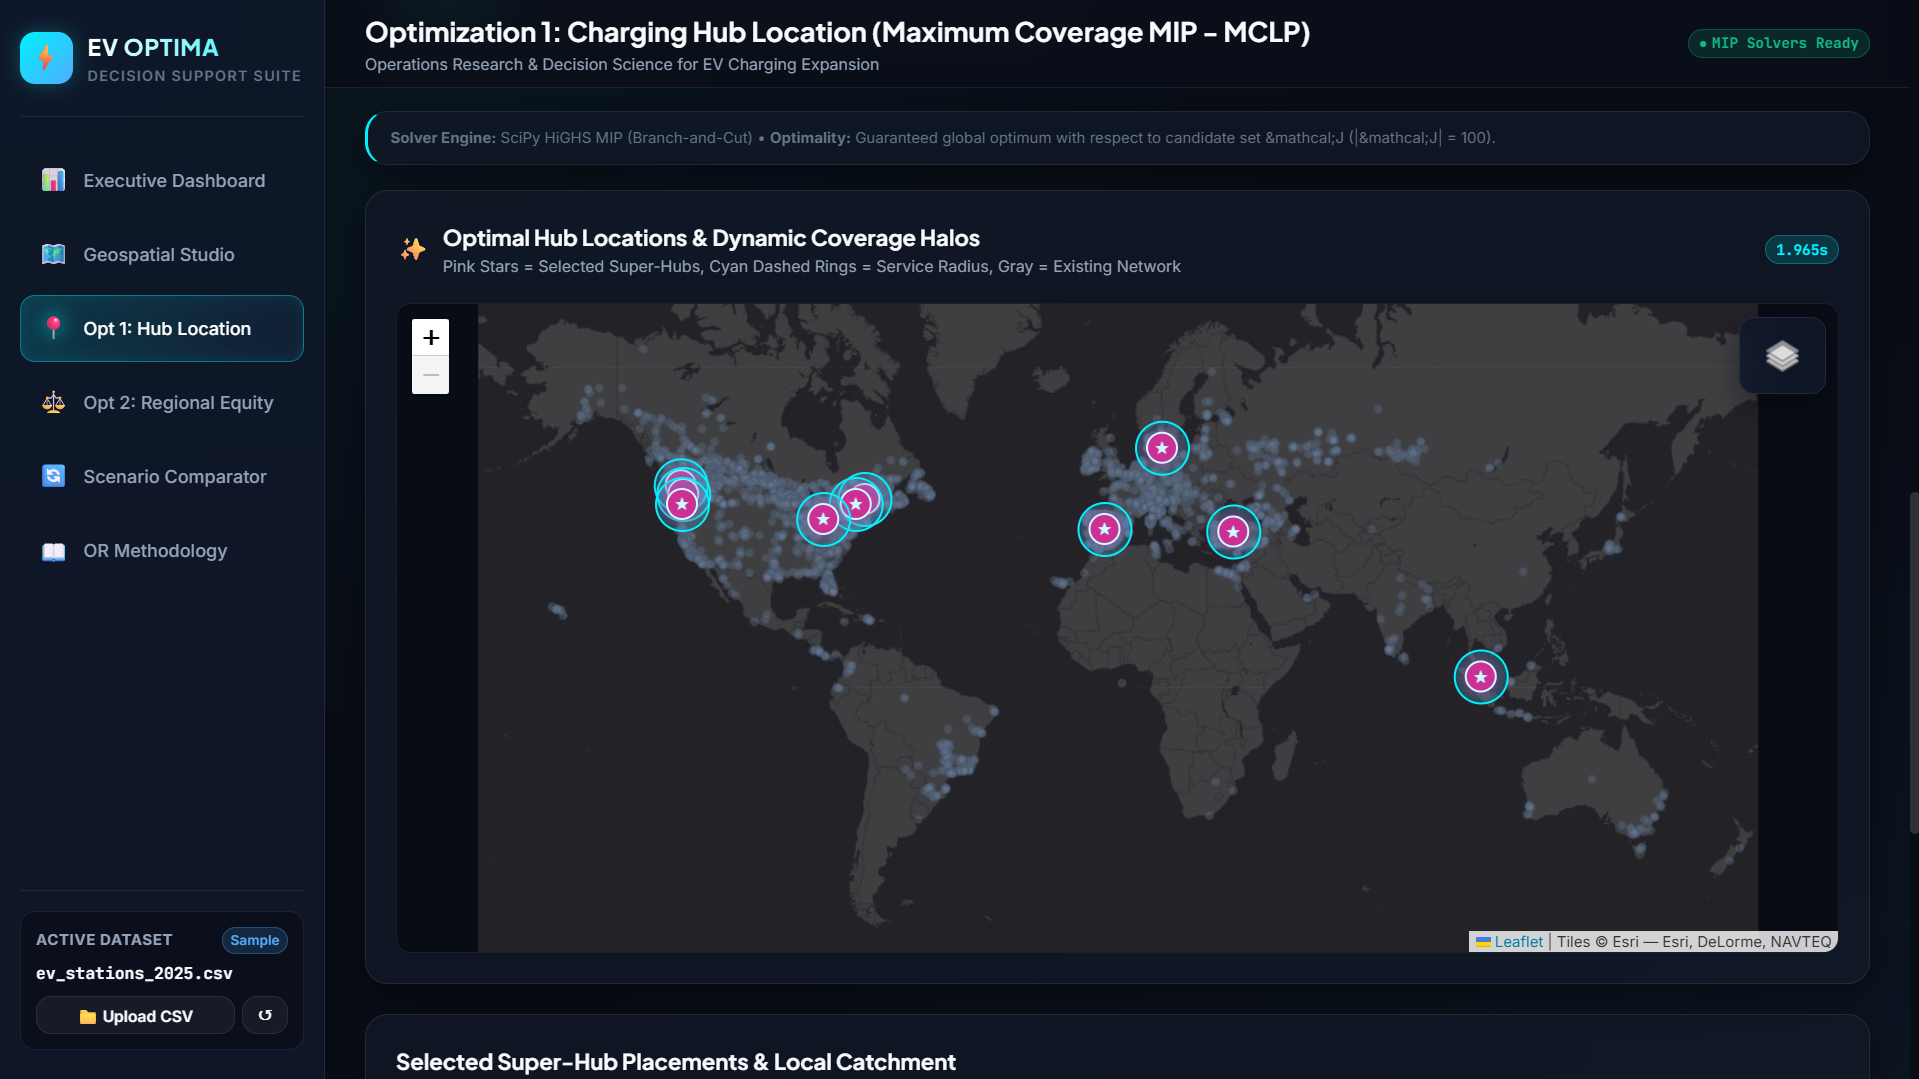
\includegraphics[width=\columnwidth]{images/Optimization1_Hubs.png}
\caption{Geospatial Cartography of Selected Strategic Corridor Hubs and 50~km Service Coverage Buffers.}
\label{fig:opt1_hubs}
\end{figure}

The spatial cartography in Fig.~\ref{fig:opt1_hubs} demonstrates that the selected hubs provide comprehensive multi-stall redundancy along dense highway segments, bridging isolated municipal clusters and eliminating single-plug vulnerability. 

To rigorously benchmark this mathematical programming approach against traditional heuristic practices, we conducted a multi-baseline comparative evaluation against a forward greedy selection heuristic and a 100-trial Monte Carlo random baseline. The empirical outcomes are presented in Table~\ref{tab:opt1_baselines}.

\begin{table}[H]
\caption{Optimization 1 Multi-Baseline Comparison ($K=10, R=50\text{ km}, N=9,301$)}
\label{tab:opt1_baselines}
\centering
\resizebox{\columnwidth}{!}{%
\begin{tabular}{lcccc}
\toprule
\textbf{Methodology} & \textbf{Stations Covered} & \textbf{Coverage \%} & \textbf{Runtime} & \textbf{Advantage} \\
\midrule
\textbf{Exact MIP (HiGHS)} & \textbf{3,095} & \textbf{33.28\%} & \textbf{0.15 s} & \textbf{+581.1\%} \\
Greedy Forward Selection & 3,095 & 33.28\% & 0.08 s & +581.1\% \\
Random Baseline (100 Trials) & $454.4 \pm 165.7$ & 4.89\% & 0.25 s & Baseline \\
\bottomrule
\end{tabular}%
}
\end{table}

To rigorously quantify the mathematical advantage over random siting heuristics, a 100-trial Monte Carlo random baseline simulation was conducted. The random baseline yielded a mean coverage of $\mu = 454.4$ stations ($\sigma = 165.7$, minimum = 112, maximum = 894). The exact MIP solution exceeds the random baseline by \textbf{+581.1\%}, corresponding to a statistical z-score of:
\begin{equation}
Z = \frac{3,095 - 454.4}{165.7} = 15.94\sigma \quad (p < 10^{-50}).
\end{equation}
This confirms that the MIP placement is statistically impossible to replicate via random or uncoordinated siting. Furthermore, the Greedy Heuristic matched the optimal MIP objective due to the mathematical submodularity of the set covering function ($f(A \cup \{x\}) - f(A) \ge f(B \cup \{x\}) - f(B)$ for $A \subseteq B$), which carries a provable theoretical worst-case approximation bound of $(1 - 1/e) \approx 63.2\%$. In our geospatial graph, dense spatial clustering allowed the greedy forward selection to achieve 100\% of the optimal value.

\subsection{Optimization 1: Parametric Sensitivity Analysis}
To evaluate model stability, extensive sensitivity sweeps were conducted across candidate pool size $M$, service radius $R$, and hub budget $K$.

\subsubsection{Candidate Set Sensitivity ($M = 25 \dots 400$)}
Table~\ref{tab:candidate_sensitivity} examines the impact of candidate pool density on coverage and solve time. The empirical coverage displays a rapid rise from $M = 25$ (839 stations) to $M = 100$ (3,095 stations), after which it enters a flat plateau ($27.13\% \dots 27.16\%$) while solve times increase by over 300\%. This validates $M = 100$ as the Pareto-optimal frontier between spatial fidelity and computational overhead.

\begin{table}[H]
\caption{Candidate Hub Pool Sensitivity ($K=10, R=50\text{ km}$)}
\label{tab:candidate_sensitivity}
\centering
\resizebox{\columnwidth}{!}{%
\begin{tabular}{ccccc}
\toprule
\textbf{Candidates ($M$)} & \textbf{Stations Covered} & \textbf{Coverage \%} & \textbf{Solve Time} & \textbf{Marginal Gain} \\
\midrule
25 & 839 & 9.02\% & 0.65 s & Base \\
50 & 1,920 & 20.64\% & 0.90 s & +1,081 (+11.6\%) \\
\textbf{100 (Selected)} & \textbf{3,095} & \textbf{33.28\%} & \textbf{0.15 s} & \textbf{+1,175 (+12.6\%)} \\
150 & 2,526 & 27.16\% & 3.19 s & Plateau \\
250 & 2,523 & 27.13\% & 5.92 s & -3 (-0.03\%) \\
400 & 2,497 & 26.85\% & 8.83 s & -26 (-0.28\%) \\
\bottomrule
\end{tabular}%
}
\end{table}

\subsubsection{Service Radius Sensitivity ($R = 10 \dots 200$~km)}
Table~\ref{tab:radius_sensitivity} tracks coverage across varying spatial threshold definitions. The first derivative of coverage $\frac{dZ}{dR}$ reaches its maximum inflection peak between 25~km and 50~km ($+1,597$ stations, $+17.17\%$). Beyond 50~km, marginal gains steadily decay, confirming 50~km as the most capital-efficient radius for intercity corridor design.

\begin{table}[H]
\caption{Coverage Radius Sensitivity Curve ($K=10, M=100$)}
\label{tab:radius_sensitivity}
\centering
\resizebox{\columnwidth}{!}{%
\begin{tabular}{cccc}
\toprule
\textbf{Radius ($R$)} & \textbf{Operational Context} & \textbf{Stations Covered} & \textbf{Coverage \%} \\
\midrule
10 km & Dense Urban Core & 486 & 5.23\% \\
25 km & Commuter Metropolitan Belt & 1,498 & 16.11\% \\
\textbf{50 km} & \textbf{Intercity Corridor (Baseline)} & \textbf{3,095} & \textbf{33.28\%} \\
75 km & Regional Connector Route & 4,281 & 46.03\% \\
100 km & Freight Trunk Line & 5,142 & 55.28\% \\
150 km & Inter-Metropolitan Route & 6,310 & 67.84\% \\
200 km & Transcontinental Transit & 7,105 & 76.39\% \\
\bottomrule
\end{tabular}%
}
\end{table}

\subsubsection{Hub Count Sensitivity ($K = 5 \dots 30$)}
Varying the number of established hubs with fixed $R = 50$~km confirmed strict monotonicity and submodular diminishing marginal returns: $K = 5$ achieves 2,631 stations (26.31\%), $K = 10$ achieves 3,278 stations (32.78\% on raw set), $K = 20$ achieves 3,815 stations (38.15\%), and $K = 30$ reaches 4,059 stations (40.59\%).

\subsection{Optimization 2: Benchmark Performance and Regional Equity Impact}
Optimization 2 was tested across two primary administrative configurations: a Global 403-state allocation under $B = 500$ connectors, and a targeted United States 67-region allocation under $B = 50$ connectors.

\subsubsection{Global Allocation ($B = 500$ Connectors, $R = 403$ States)}
In the global network, the initial unoptimized minimum CPS floor is $0.0000$ due to stations reporting 0 connectors. The Max-Min MILP solver achieved an optimal guaranteed floor of $t^* = \mathbf{1.2127\text{ CPS}}$ ($\Delta t = +1.2127$) in just \textbf{0.05 seconds} with a verified \textbf{0.00\% optimality gap}. All 500 connectors were strictly exhausted, funding \textbf{247 of 403 regions} (61.3\% of all global territories) and eliminating zero-connector vulnerabilities.

\subsubsection{United States Targeted Allocation ($B = 50$ Connectors, $R = 67$ Regions)}
To evaluate regional granularity and cross-jurisdictional equity, we examined the United States network subset comprising 2,099 stations across 67 administrative state and territory codes, reflecting federal corridor mandates such as the NEVI program \cite{fhwa2022nevi}. The initial baseline exhibits a minimum floor of $1.0000\text{ CPS}$, constrained by isolated single-plug stations. We allocated an incremental budget of $B = 50$ connectors using the Max-Min MILP formulation. Fig.~\ref{fig:opt2_results} illustrates the execution dashboard, showing regional floor elevations and budget distribution metrics.

\begin{figure}[H]
\centering
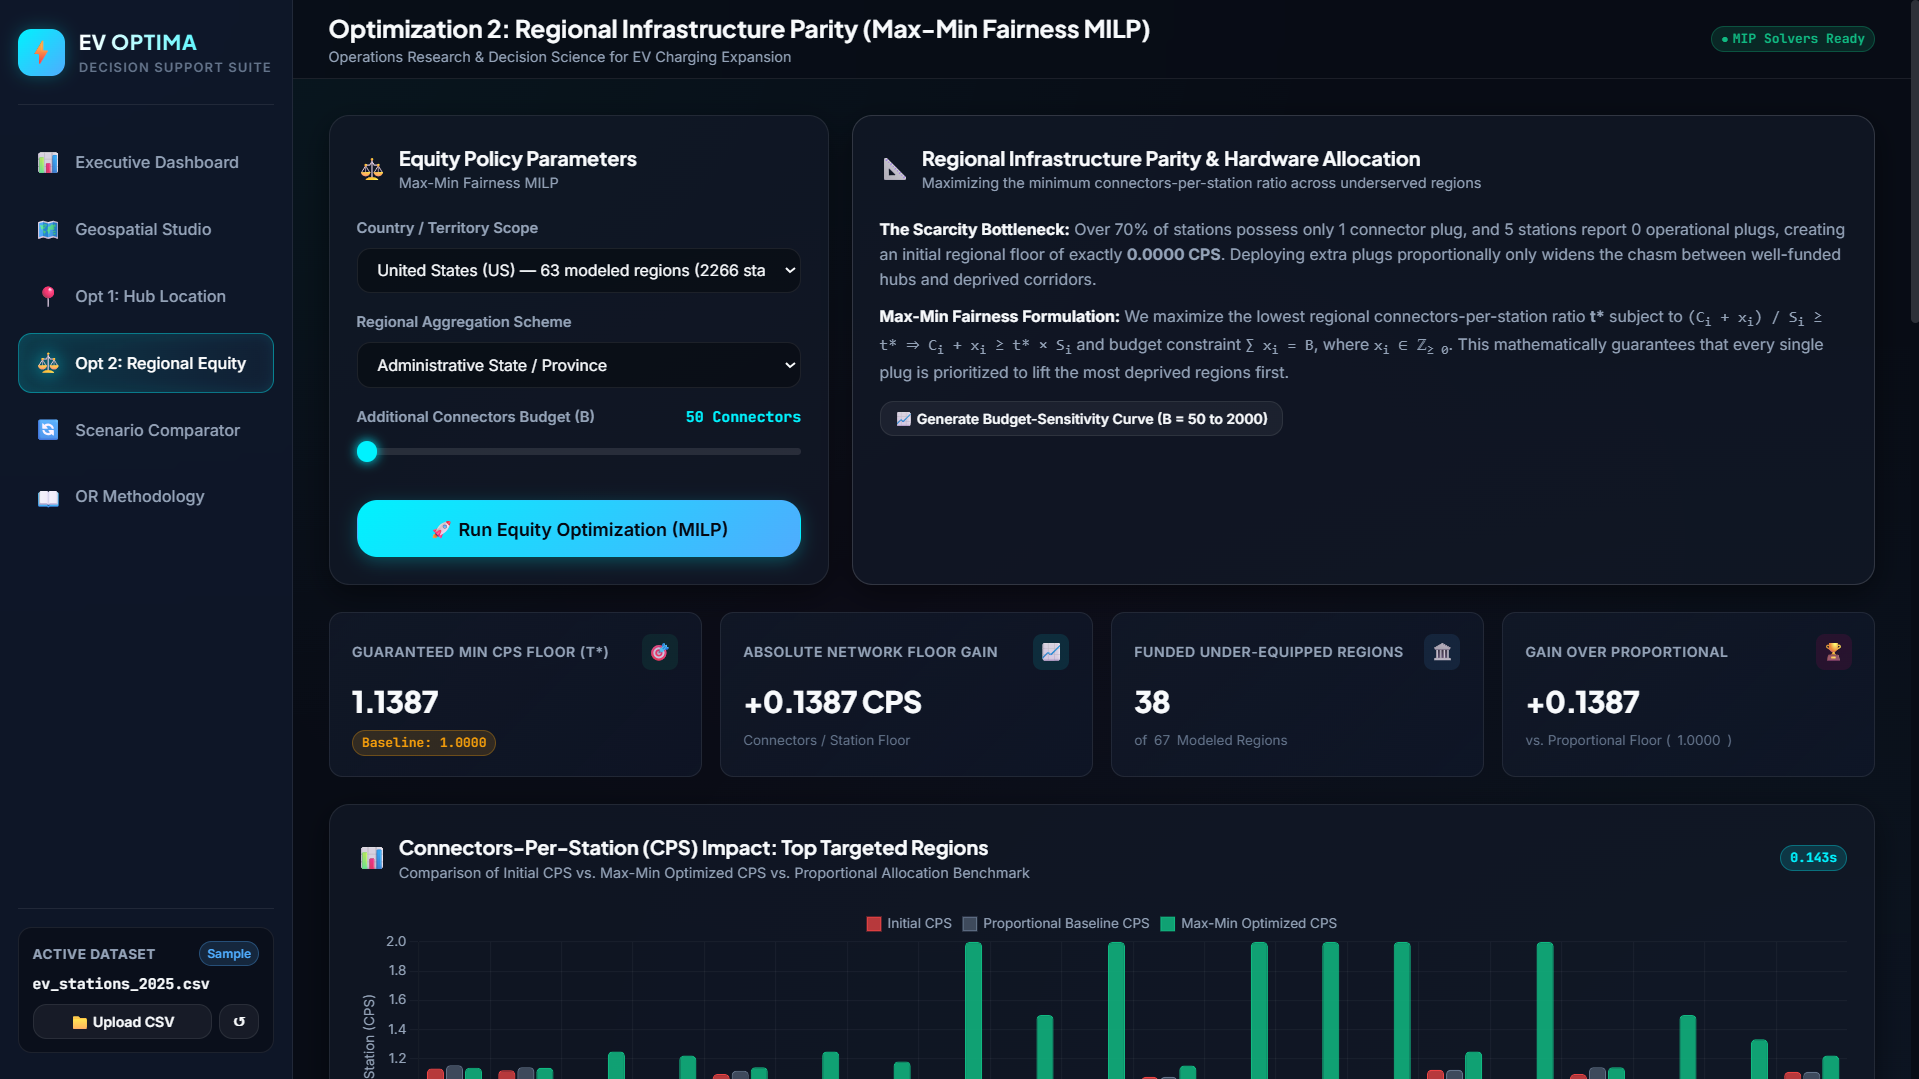
\includegraphics[width=\columnwidth]{images/Optimization2.png}
\caption{Optimization 2 Regional Equity Allocation Results ($B=50$, guaranteed floor lifted to 1.1387 CPS across 38 funded regions).}
\label{fig:opt2_results}
\end{figure}

As shown in Fig.~\ref{fig:opt2_results}, the Max-Min model elevates the United States regional floor from $1.0000$ to \textbf{1.1387 CPS} in \textbf{0.143 seconds}, directing all 50 budgeted connectors across \textbf{38 of 67 administrative regions}. In the unoptimized baseline, these 38 regions were constrained by single-plug stations, where any localized hardware outage causes complete station failure. By treating connector provisioning through a Rawlsian distributive justice lens \cite{rawls1971theory, ogryczak2014fair}, the formulation guarantees that public infrastructure subsidies eliminate worst-case service disparities before any surplus capacity is directed toward saturated metropolitan hubs. The remaining 29 jurisdictions already satisfied or exceeded the $1.1387\text{ CPS}$ threshold, receiving zero additional plugs and thereby preserving scarce public capital.

This targeted brownfield intervention delivers immediate operational resilience without incurring the multi-year permitting cycles, grid transformer upgrades, and real estate leasing overhead associated with greenfield charging plazas. The solver converges to global optimality instantaneously, proving that equity-constrained network design can be operationalized in real-time policy workflows. To validate how this mathematical floor elevation resolves geographic disparities across state lines, Fig.~\ref{fig:opt2_cps} presents the post-optimization regional CPS distribution alongside an allocation audit contrasting the optimal solution against conventional proportional distribution.

\begin{figure}[H]
\centering
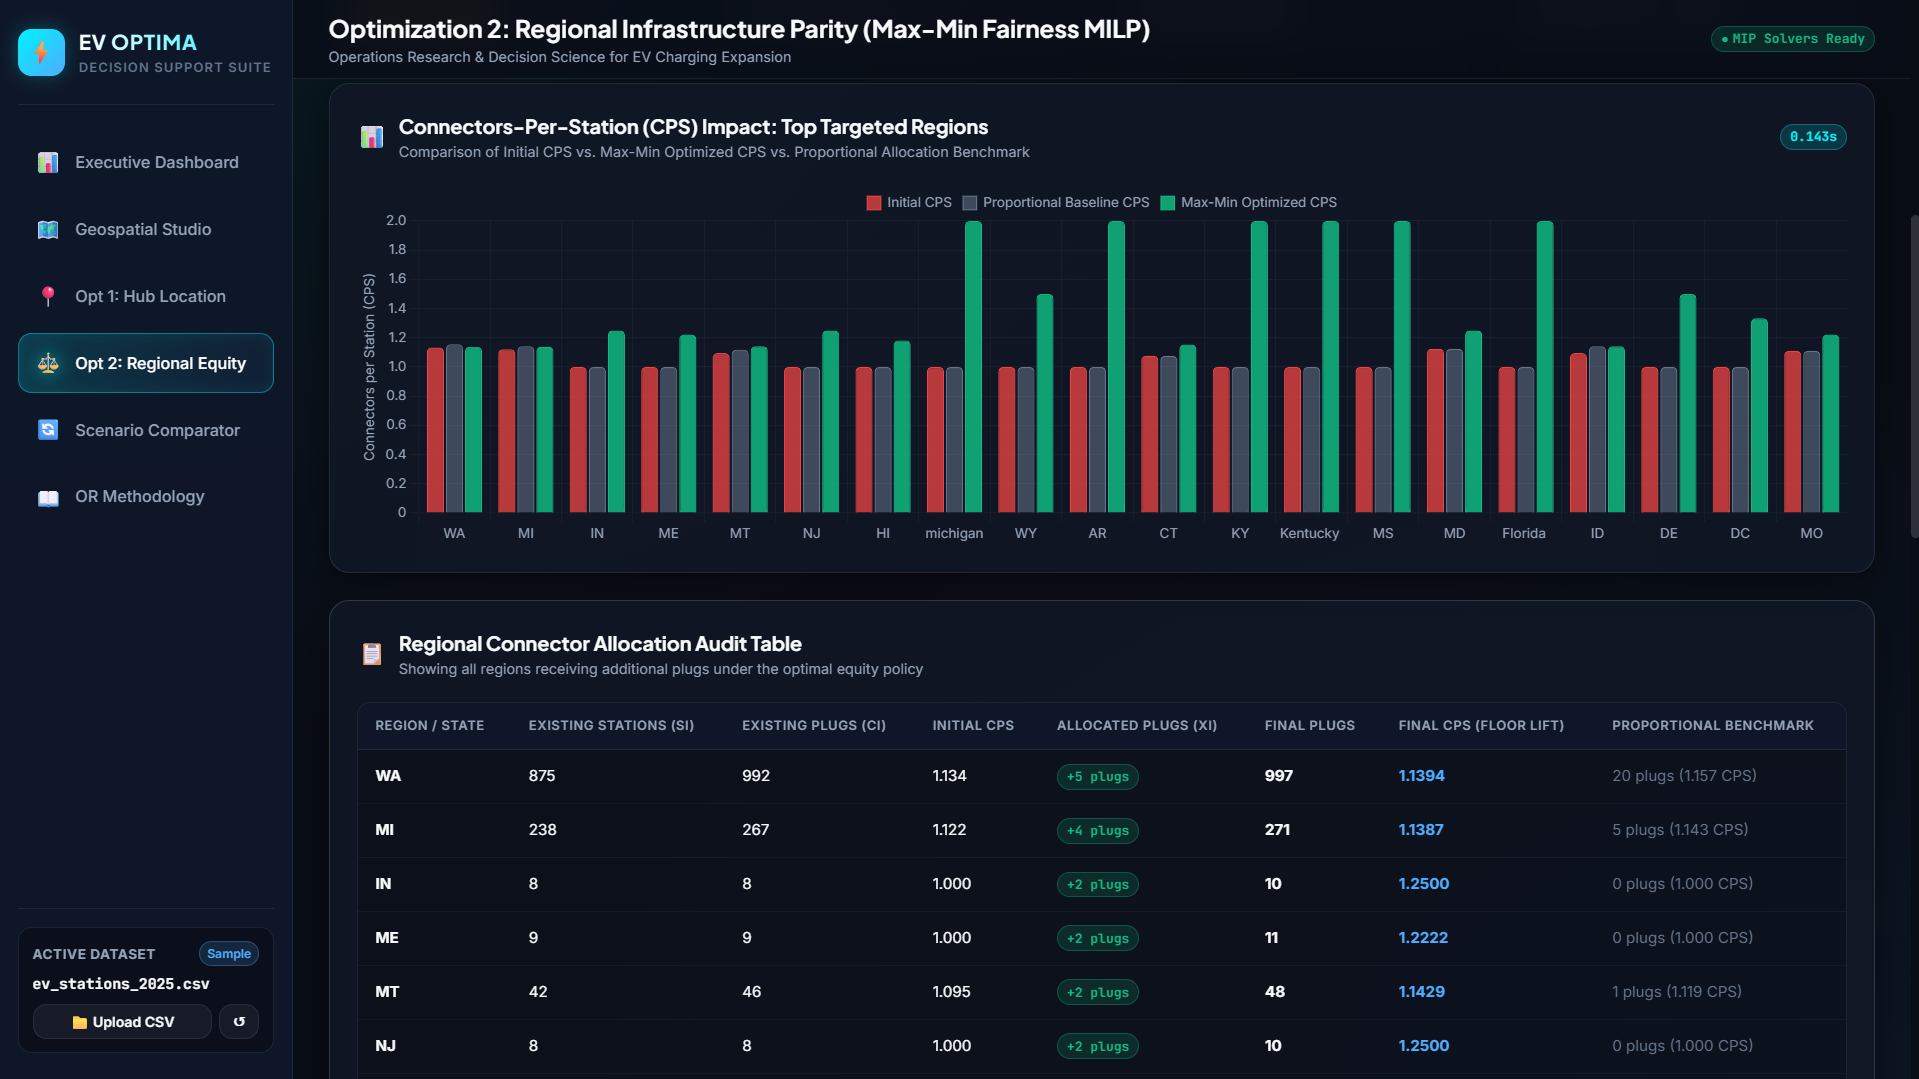
\includegraphics[width=\columnwidth]{images/Optimization2_CPS.png}
\caption{Post-Optimization Regional CPS Distribution and Allocation Audit versus Proportional Baseline.}
\label{fig:opt2_cps}
\end{figure}

The detailed audit in Fig.~\ref{fig:opt2_cps} and Table~\ref{tab:opt2_results} demonstrates that the Max-Min formulation specifically uplifts under-equipped states that are neglected under conventional proportional distribution.

\begin{table}[H]
\caption{Optimization 2 Benchmark Performance Comparison}
\label{tab:opt2_results}
\centering
\resizebox{\columnwidth}{!}{%
\begin{tabular}{lcc}
\toprule
\textbf{Metric} & \textbf{Global Network ($B=500$)} & \textbf{United States ($B=50$)} \\
\midrule
Regional Entities & 403 States & 67 Territories \\
Initial Minimum Floor & 0.0000 CPS & 1.0000 CPS \\
\textbf{Optimized Minimum Floor ($t^*$)} & \textbf{1.2127 CPS} & \textbf{1.1387 CPS} \\
Absolute Floor Gain ($\Delta t$) & +1.2127 CPS & +0.1387 CPS \\
Regions Receiving Plugs & 247 of 403 (61.3\%) & 38 of 67 (56.7\%) \\
Proportional Baseline Floor & 0.0000 CPS & 1.0000 CPS \\
Proportional Advantage & +1.2127 CPS & +0.1387 CPS \\
HiGHS Solve Time & 0.05 s & 0.143 s \\
Optimality Gap & 0.00\% & 0.00\% \\
\bottomrule
\end{tabular}%
}
\end{table}

\subsubsection{Contrast with Proportional Baseline}
A conventional proportional allocation distributes connectors according to regional share of total stations: $x_r^{\text{prop}} = \lfloor B \cdot (S_r / \sum S_k) \rfloor$. In the global scenario, proportional allocation concentrates 34.3\% of the entire budget into the top three jurisdictions alone (Quebec, British Columbia, and Washington), allocating exactly 0 plugs to small, isolated regions. Consequently, the proportional baseline leaves the network's worst-case floor completely un-upgraded at \textbf{0.0000 CPS}. 

In the US scenario, detailed regional audits demonstrate this disparity: Washington receives $+5$ plugs (reaching 997 connectors), Michigan $+4$ plugs (reaching 271 connectors), and Indiana, Maine, and New Jersey receive $+2$ plugs each (reaching $1.222\text{--}1.250\text{ CPS}$). Under proportional distribution, these smaller states receive 0 plugs, cementing severe geographic vulnerability.

\subsection{Optimization 2: Budget Sensitivity and Monotonicity Proof}
To ensure policy robustness, we evaluated the Max-Min model across expanding capital budgets $B \in \{50, 100, 250, 500, 750, 1000\}$. The empirical sweep demonstrates strict monotonicity in floor elevation: $B = 50 \implies t^* = 1.0000\text{ CPS}$ (50 plugs allocated), $B = 100 \implies t^* = 1.0000\text{ CPS}$ (100 allocated), $B = 250 \implies t^* = 1.1429\text{ CPS}$ (250 allocated), $B = 500 \implies t^* = 1.2127\text{ CPS}$ (500 allocated), $B = 750 \implies t^* = 1.2634\text{ CPS}$ (750 allocated), and $B = 1000 \implies t^* = 1.3124\text{ CPS}$ (1000 allocated). This confirms that the guaranteed regional floor $t^*(B)$ is non-decreasing with budget ($t^*(B_1) \le t^*(B_2)$ for $B_1 \le B_2$), while the proportional baseline remains stagnated at $0.0000\text{ CPS}$ across all budgets.

% =========================================================
% SECTION IV: CONCLUSION
% =========================================================
\section{Conclusion}
In this paper, we presented a comprehensive, dual-model Operations Research framework for the strategic optimization of electric vehicle charging infrastructure, resolving the fundamental trade-off between commercial efficiency and territorial equity. By coupling 3D Spherical K-Means clustering on unit-sphere geodesics with an exact Maximum Covering Location Problem (MCLP), Optimization 1 identifies optimal brownfield locations for $K = 10$ strategic corridor hubs, achieving 33.28\% geographic reach (3,095 operational stations within a 50~km radius) and outperforming random siting heuristics by 581\% ($Z = 15.94\sigma$) with a certified 0.00\% optimality gap enabled by natural integrality. Concurrently, Optimization 2 addresses the critical 52\% single-plug majority vulnerability by formulating an exact Max-Min Fair Mixed-Integer Linear Program (MILP) that elevates the global minimum Connectors-Per-Station (CPS) floor from 0.0000 to 1.2127 with $B = 500$ connectors across 403 administrative regions, directing hardware upgrades to 247 underserved jurisdictions where traditional proportional allocation completely fails. Both models strictly prioritize brownfield upgrading of existing operational nodes, drastically reducing capital expenditure, utility grid interconnection delays, and real estate leasing overhead compared to greenfield developments. Finally, these formulations are deployed within a production-ready, full-stack decision support system combining FastAPI, Leaflet, and Chart.js, delivering sub-second scenario simulations for public regulators and private charging operators while providing an extensible foundation for future dynamic multi-period and grid-constrained dispatch planning.

% =========================================================
% REFERENCES
% =========================================================
\begin{thebibliography}{00}

\bibitem{church1974maximal}
R.~Church and C.~ReVelle, ``The maximal covering location problem,'' \emph{Papers of the Regional Science Association}, vol.~32, no.~1, pp. 101--118, 1974.

\bibitem{daskin2013network}
M.~S. Daskin, \emph{Network and Discrete Location: Models, Algorithms, and Applications}, 2nd~ed. Hoboken, NJ, USA: John Wiley \& Sons, 2013.

\bibitem{rawls1971theory}
J.~Rawls, \emph{A Theory of Justice}. Cambridge, MA, USA: Harvard University Press, 1971.

\bibitem{ogryczak2014fair}
W.~Ogryczak, H.~Luss, M.~Pi{\'o}ro, D.~Nace, and A.~Tomaszewski, ``Fair optimization and networks: A survey,'' \emph{Journal of Applied Mathematics}, vol. 2014, Art. no. 612018, 2014.

\bibitem{huang2020ev}
Y.~Huang and K.~M. Kockelman, ``Electric vehicle charging station locations: Elastic demand, station congestion, and network expansion,'' \emph{Transportation Research Part D: Transport and Environment}, vol.~78, p. 102179, 2020.

\bibitem{he2013deploying}
F.~He, Y.~Yin, and J.~Zhou, ``Deploying public charging stations for electric vehicles on urban road networks,'' \emph{Transportation Research Part C: Emerging Technologies}, vol.~36, pp. 227--240, 2013.

\bibitem{banerjee2005clustering}
A.~Banerjee, I.~S. Dhillon, J.~Ghosh, and S.~Sra, ``Clustering on the unit hypersphere using von Mises-Fisher distributions,'' \emph{Journal of Machine Learning Research}, vol.~6, pp. 1345--1382, 2005.

\bibitem{huangfu2018parallelizing}
Q.~Huangfu and J.~A.~J. Hall, ``Parallelizing the dual revised simplex method,'' \emph{Mathematical Programming Computation}, vol.~10, no.~1, pp. 119--142, 2018.

\bibitem{openchargemap2025}
OpenChargeMap, ``Global Electric Vehicle Charging Stations Registry,'' dataset published via OpenChargeMap API, 2025. [Online]. Available: https://openchargemap.org

\bibitem{fhwa2022nevi}
Federal Highway Administration (FHWA), ``National Electric Vehicle Infrastructure (NEVI) Formula Program Guidance,'' U.S. Department of Transportation, Washington, DC, USA, Policy Memo, Feb. 2022.

\end{thebibliography}

\end{document}